\chapter{Usage and experimentation} \label{chap:usage}

\section*{}

In this chapter it is presented an usage example of the created prototype. It is also presented too a comparison between a manual evaluation and an evaluation generated by this tool.

\section{Usage example} \label{sec:usageexample}
	%Usage example - Dar um exemplo de utilização com printscrn

To demonstrate the prototype it is presented in this section an usage example of the created methodologies and rules.

As said before all of this was implemented inside Scraim, so its usage is restricted to users that have an account on Scraim with this module enabled.

\vspace{10 mm}

\textbf{Home Screen}

So if a user that is registered in Scraim logs in, on the side bar of Scraim (its menu) is possible to see the assessment logo. By clicking on that logo, the user is directed to the assessments module homepage, presented in Figure \ref{fig:no_assessments}.

\begin{figure}[!htb]
	\begin{center}
		\leavevmode
		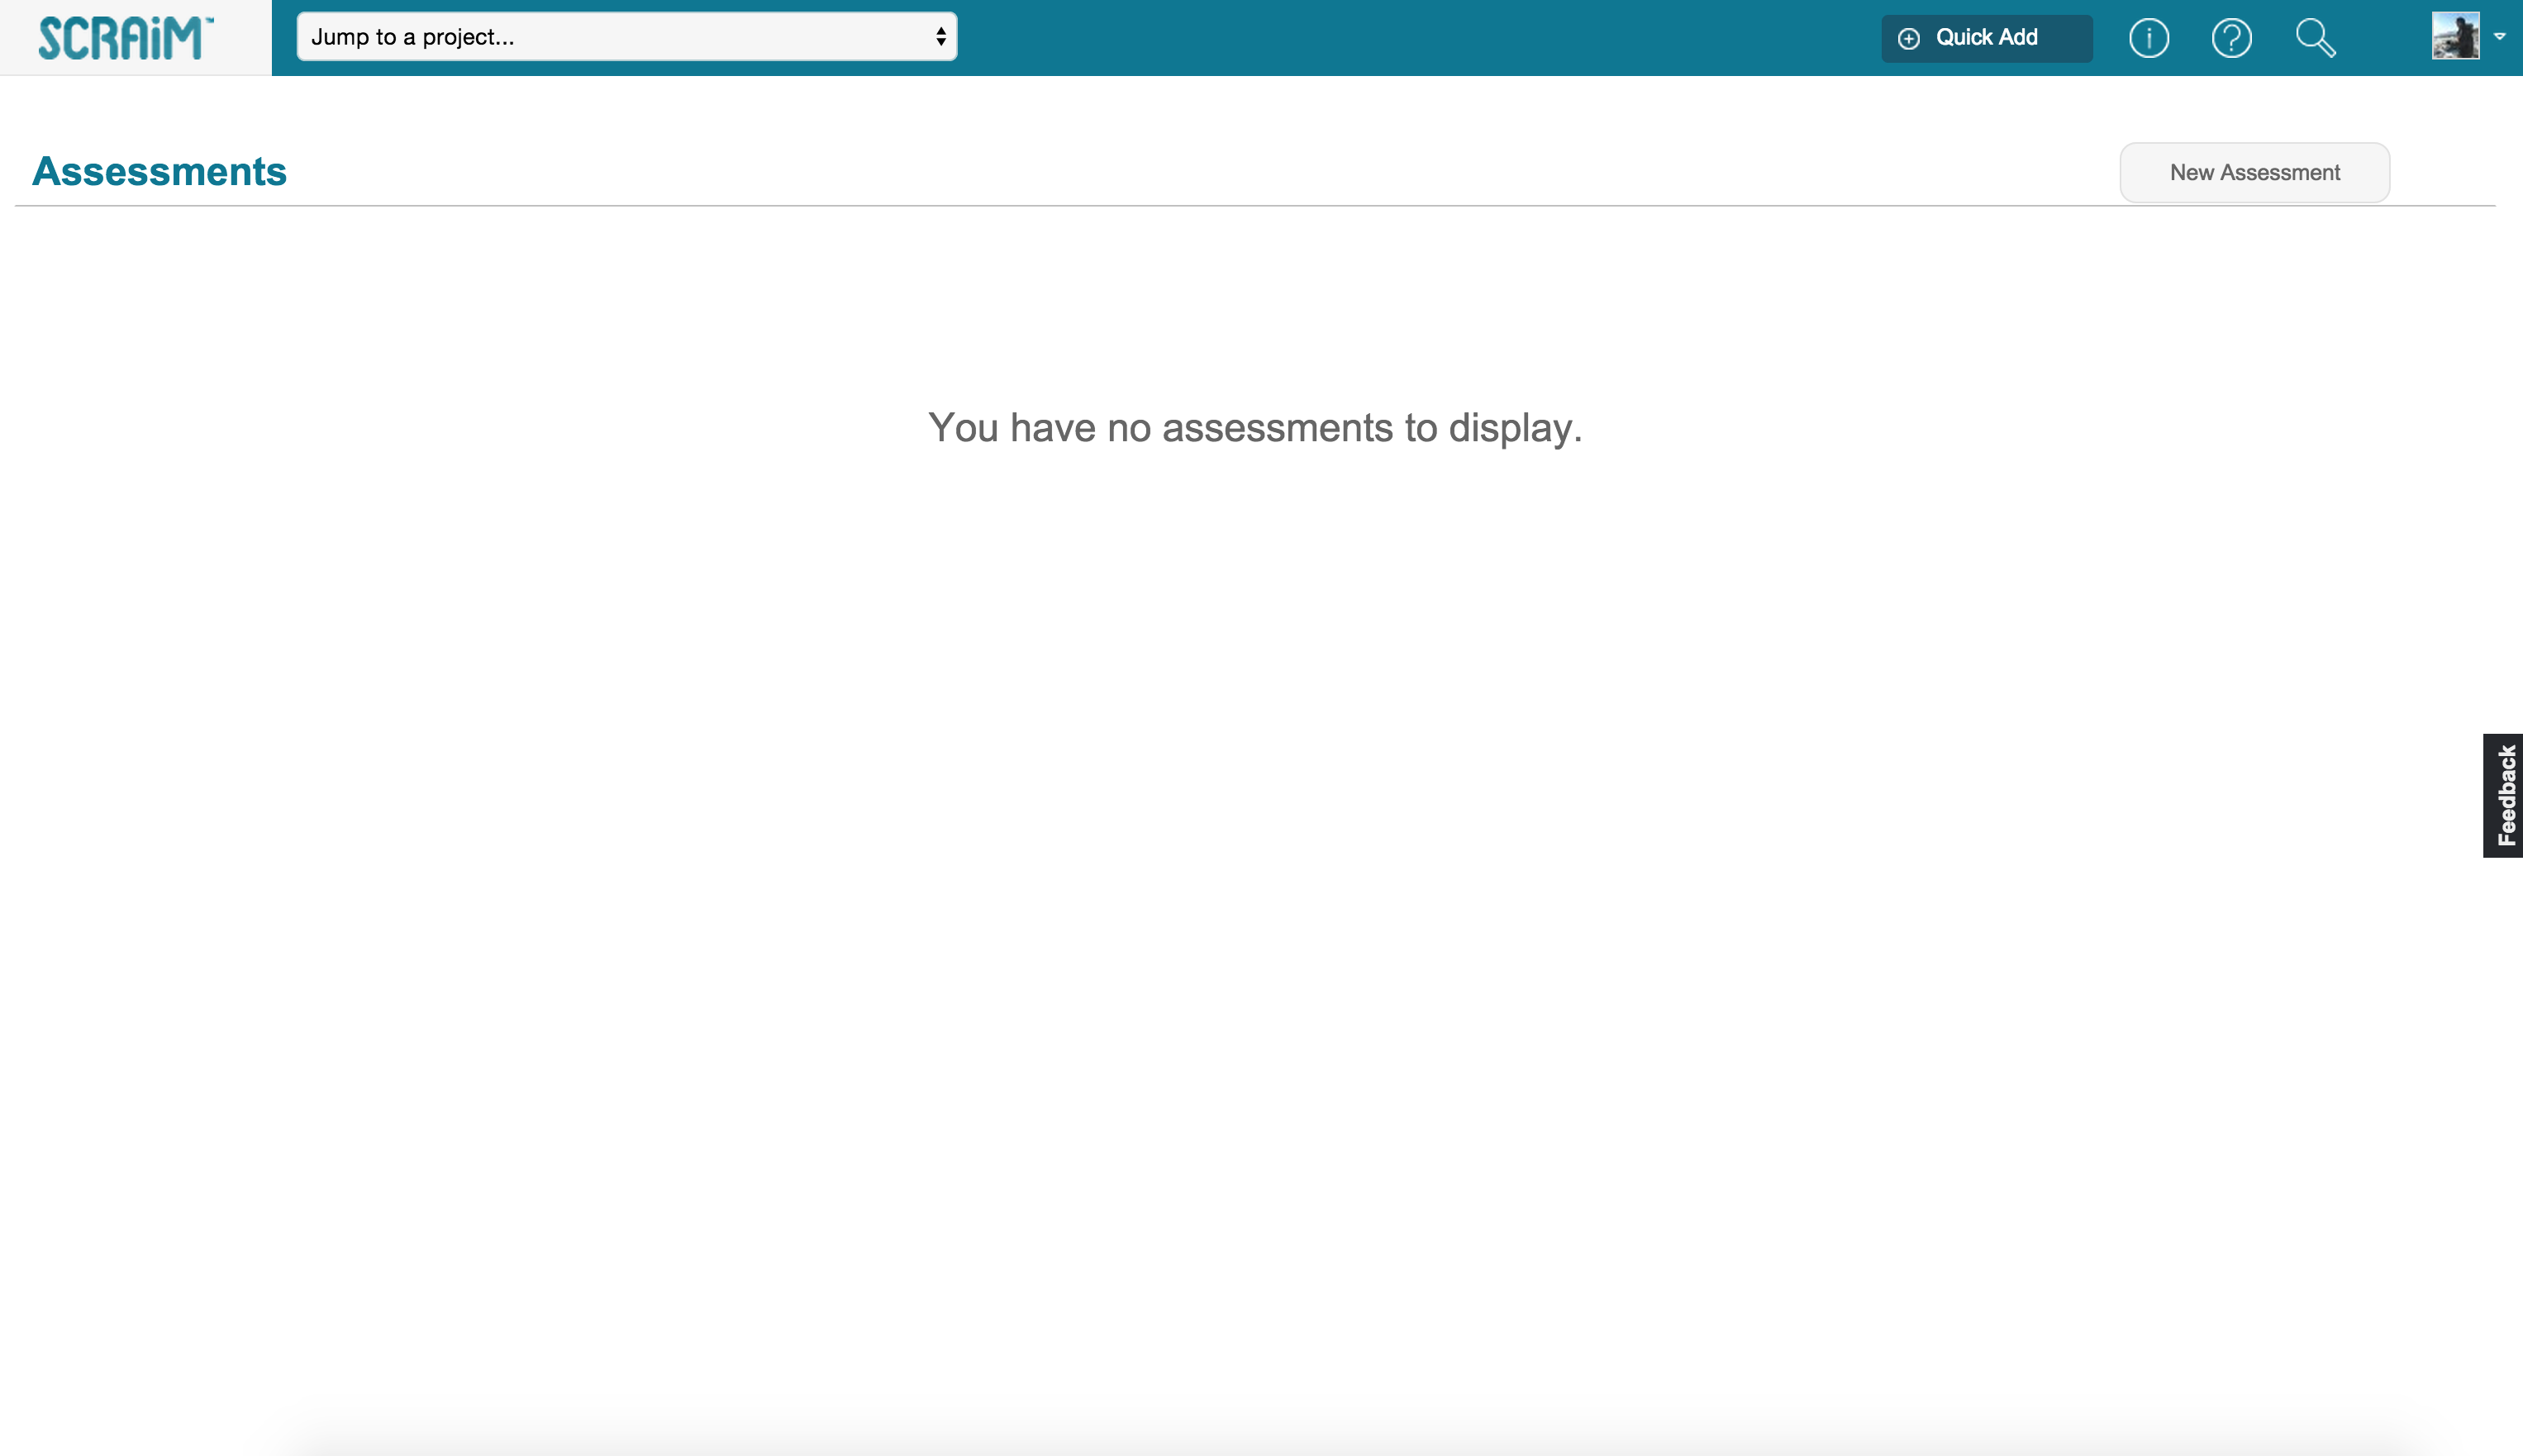
\includegraphics[width=0.9\textwidth]{no_assessments}
		\caption{Homepage without assessments done}
		\label{fig:no_assessments}
	\end{center}
\end{figure}

This screen is shown when we don't have assessments performed. If there are some assessments done in this screen is presented a list of the assessments, as shown in Figure \ref{fig:done_assessments}. In the Image, the three assessments are shown by chronological order, with the most recent assessments on the bottom.

\begin{figure}[!htb]
	\begin{center}
		\leavevmode
		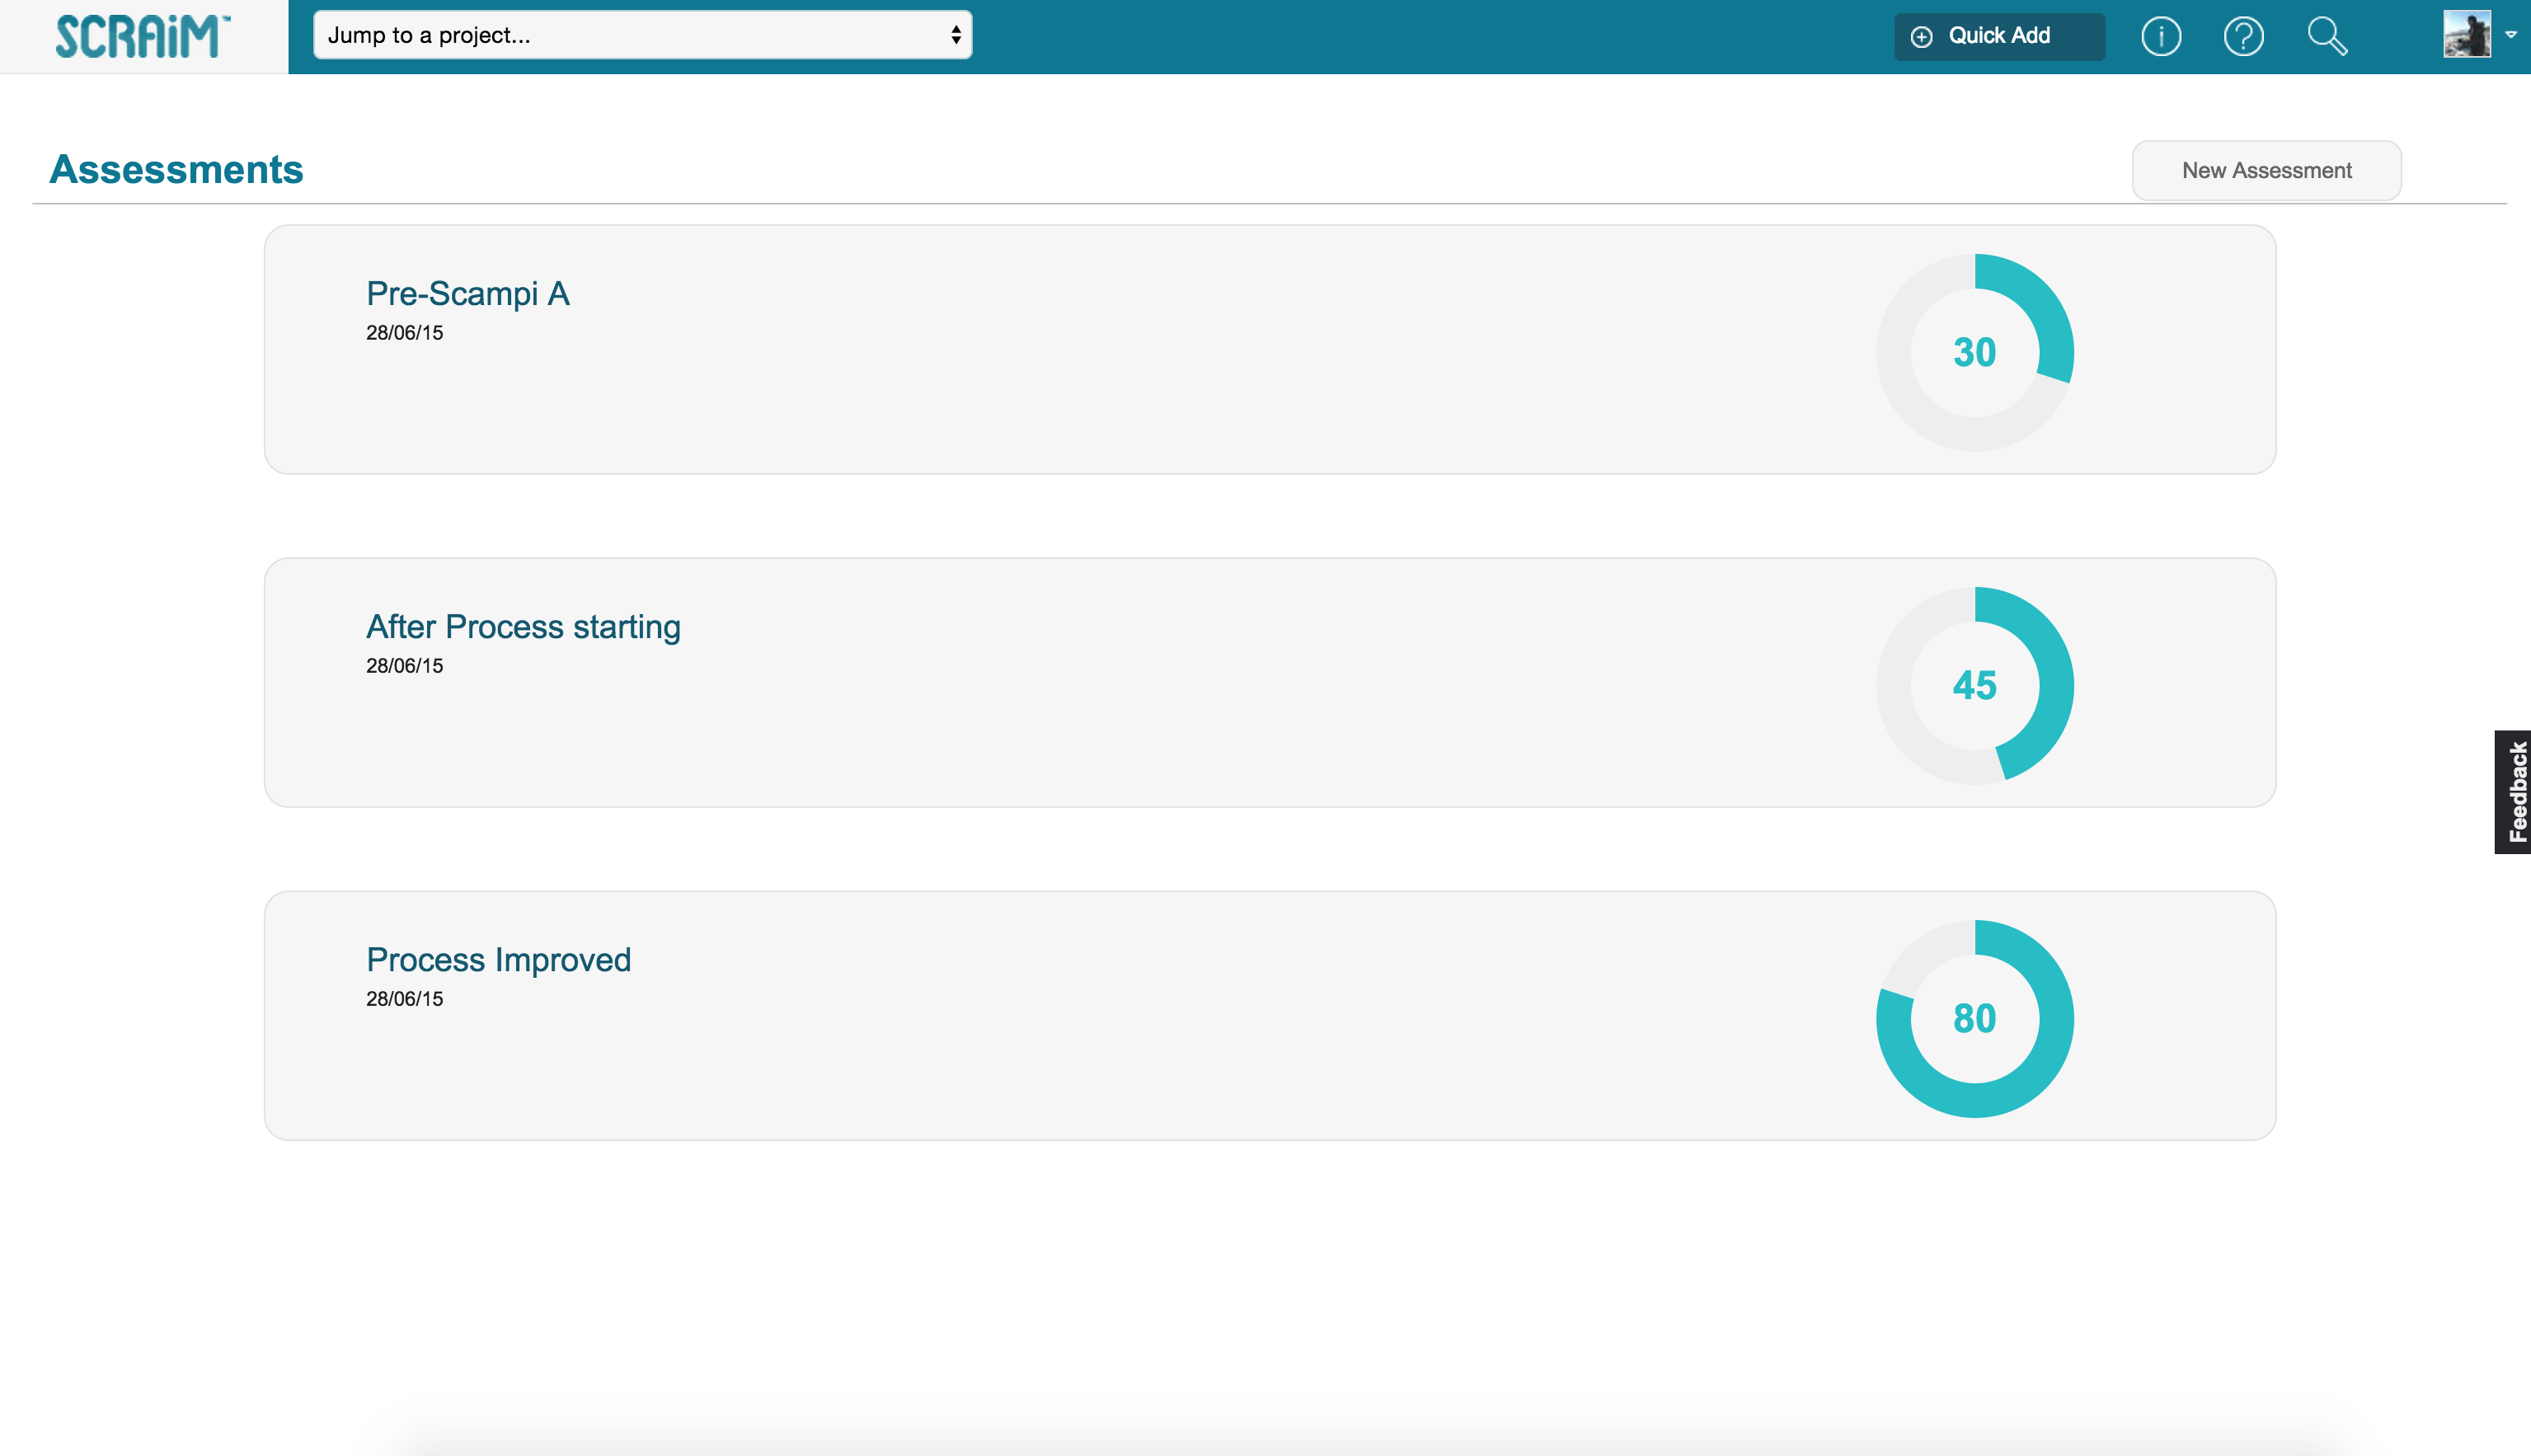
\includegraphics[width=0.9\textwidth]{done_assessments}
		\caption{Homepage with three assessments done}
		\label{fig:done_assessments}
	\end{center}
\end{figure}


\vspace{10 mm}

\textbf{Assessment Options}

In Figure \ref{fig:done_assessments}, on the right top corner there is a button entitled "New assessment". When that button is pressed the application leads the user to a screen where is prepared the assessment. This preparation screen can be seen in Figure \ref{fig:prepare_assessment}; in this page the user may specify a custom name for the assessment. If the name is not specified a automatic name will be generated with the date and time of the assessment. Additionally, the user has to choose the project or projects that are going to be evaluated.

\begin{figure}[!htb]
	\begin{center}
		\leavevmode
		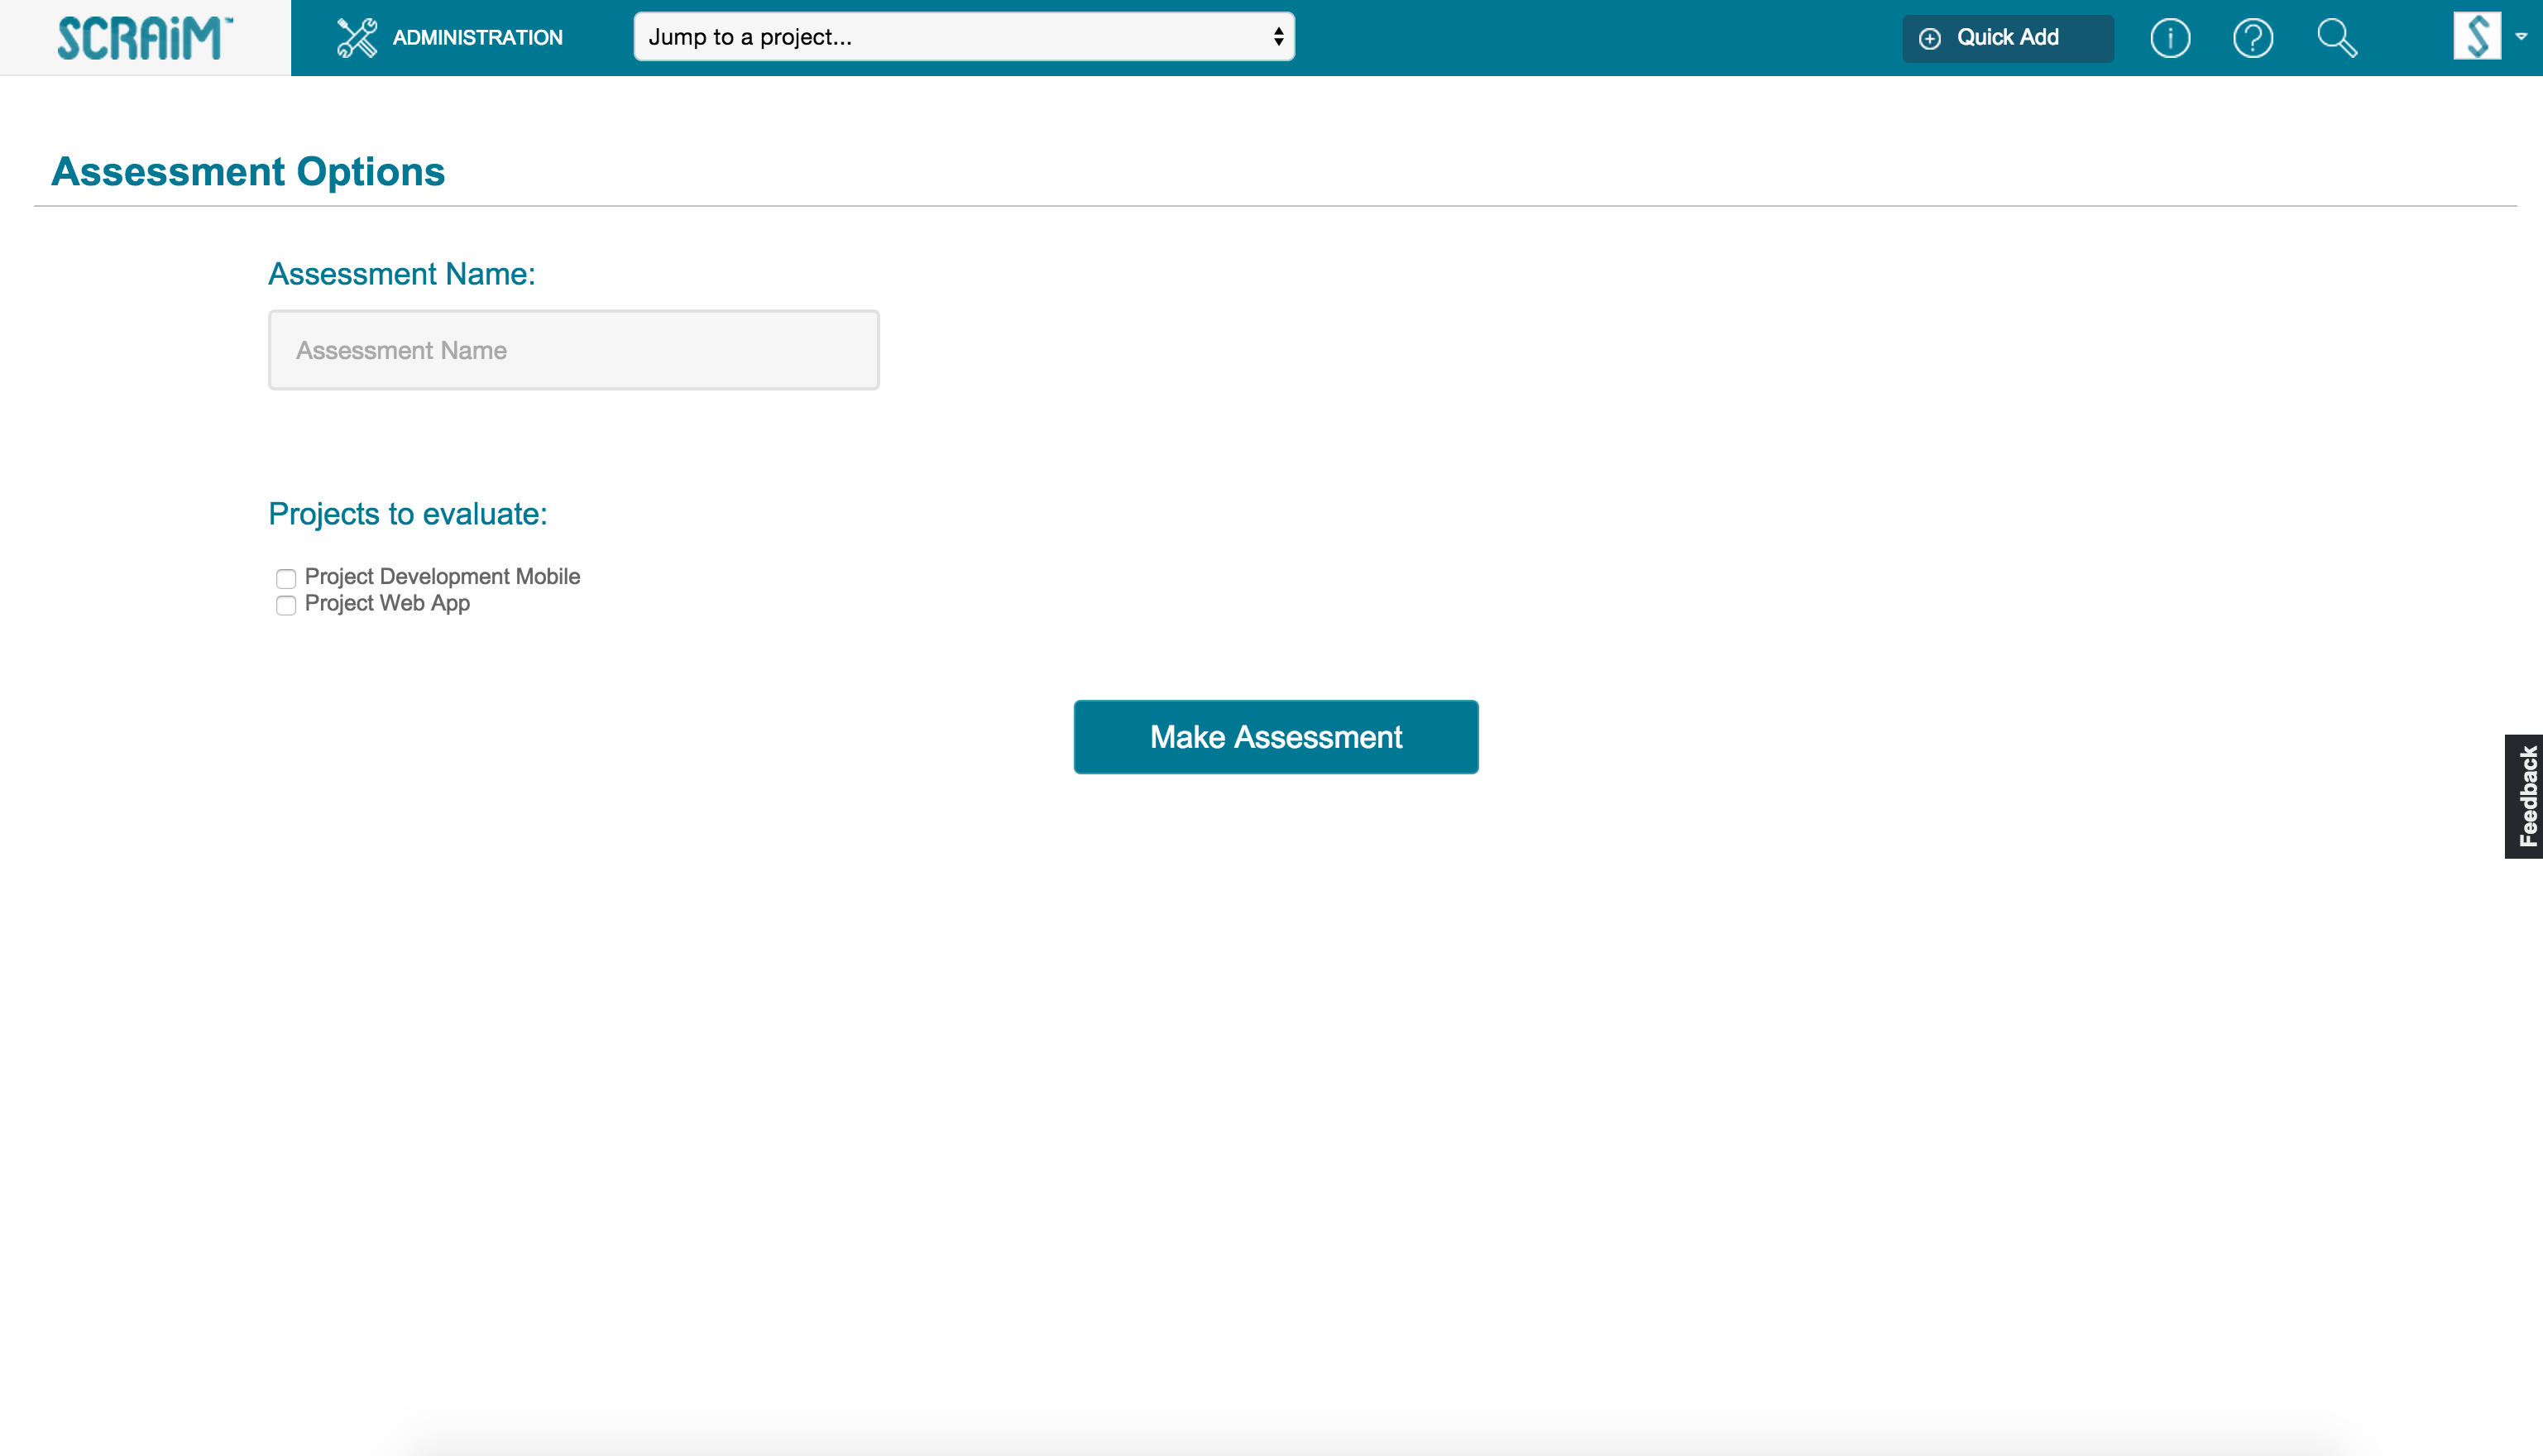
\includegraphics[width=0.9\textwidth]{prepare_assessment}
		\caption{Assessment Preparation}
		\label{fig:prepare_assessment}
	\end{center}
\end{figure}

Only the text field can be empty, is mandatory to choose at least one project. After completing this process, the button "Make Assessment" can be clicked leading to the screen presented in Figure \ref{fig:goto_survey}.

\vspace{10 mm}

\textbf{Survey}

\begin{figure}[!htb]
	\begin{center}
		\leavevmode
		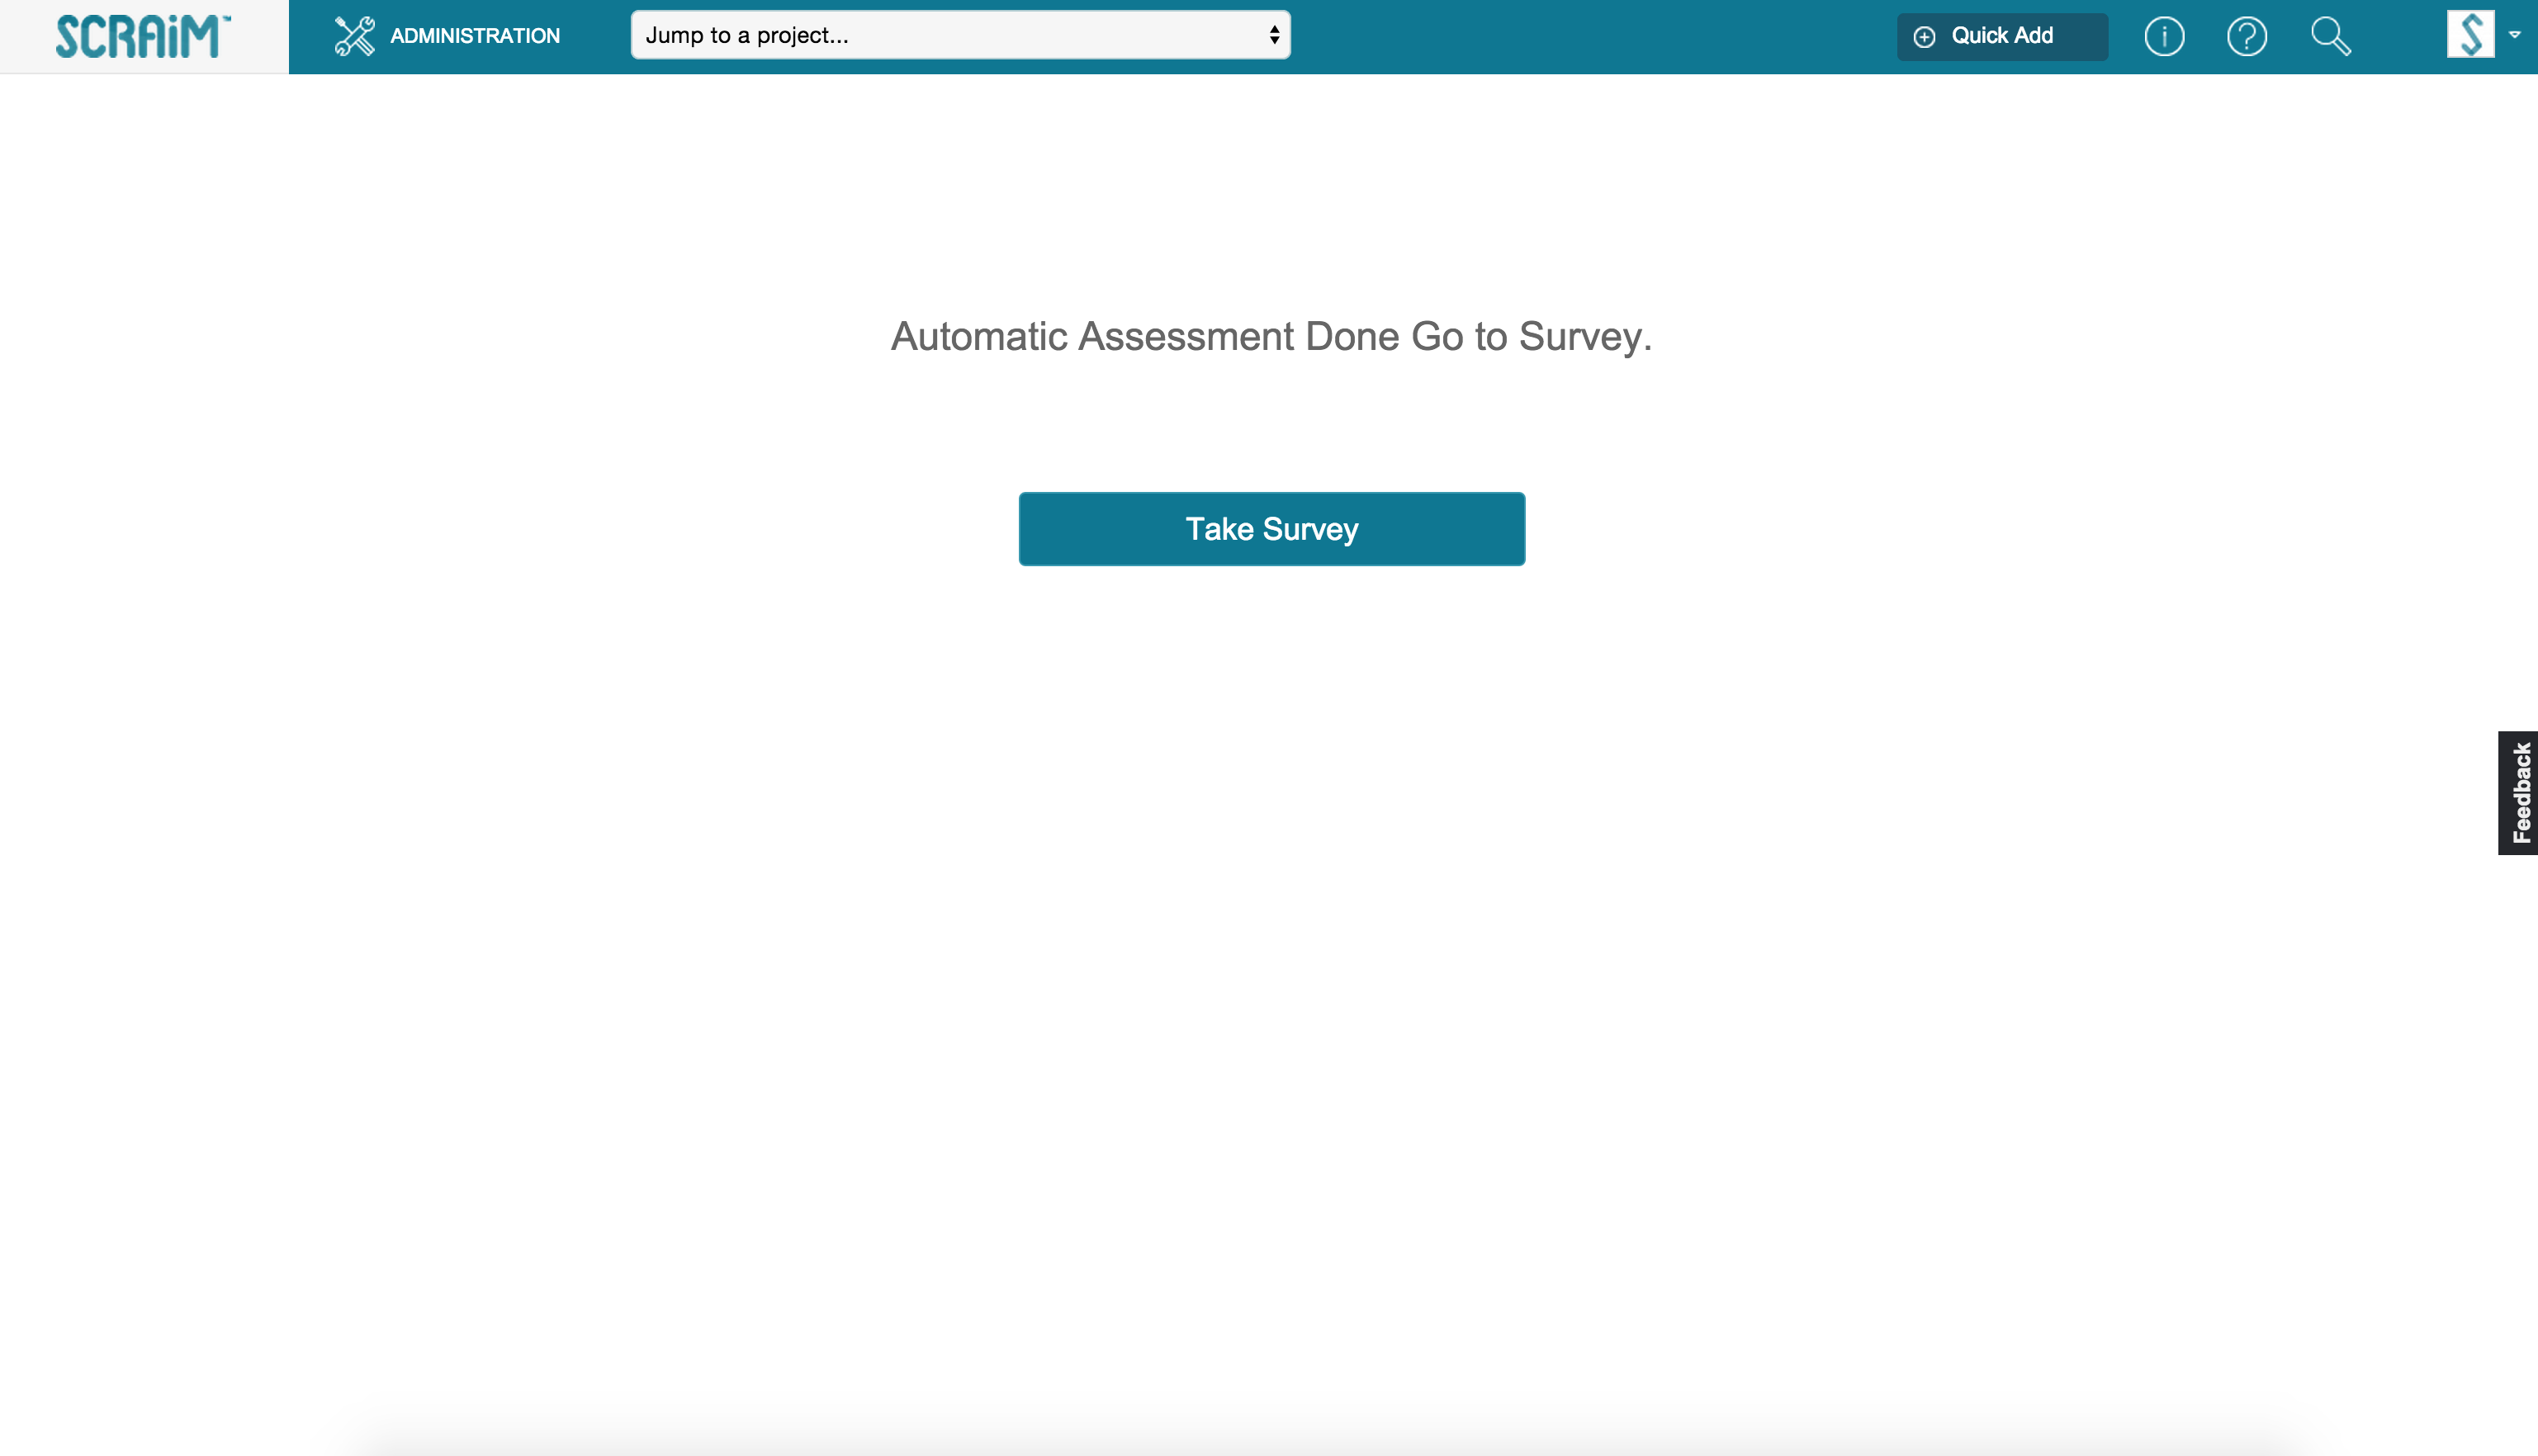
\includegraphics[width=0.9\textwidth]{goto_survey}
		\caption{After Automatic Assessment, needed Survey}
		\label{fig:goto_survey}
	\end{center}
\end{figure}

The Survey is the Screen where is needed to answer all the questions, none can be skipped and only after that we can have a full assessment done and a proper result.

\vspace{10 mm}

\textbf{Results}

When all the process is completed we can see the results obtained, as illustrated in Figure \ref{fig:area_view}. In this screen we can see the result of a project per process area. In this case, only two process areas are evaluated (PMC and PP).

\begin{figure}[h]
	\begin{center}
		\leavevmode
		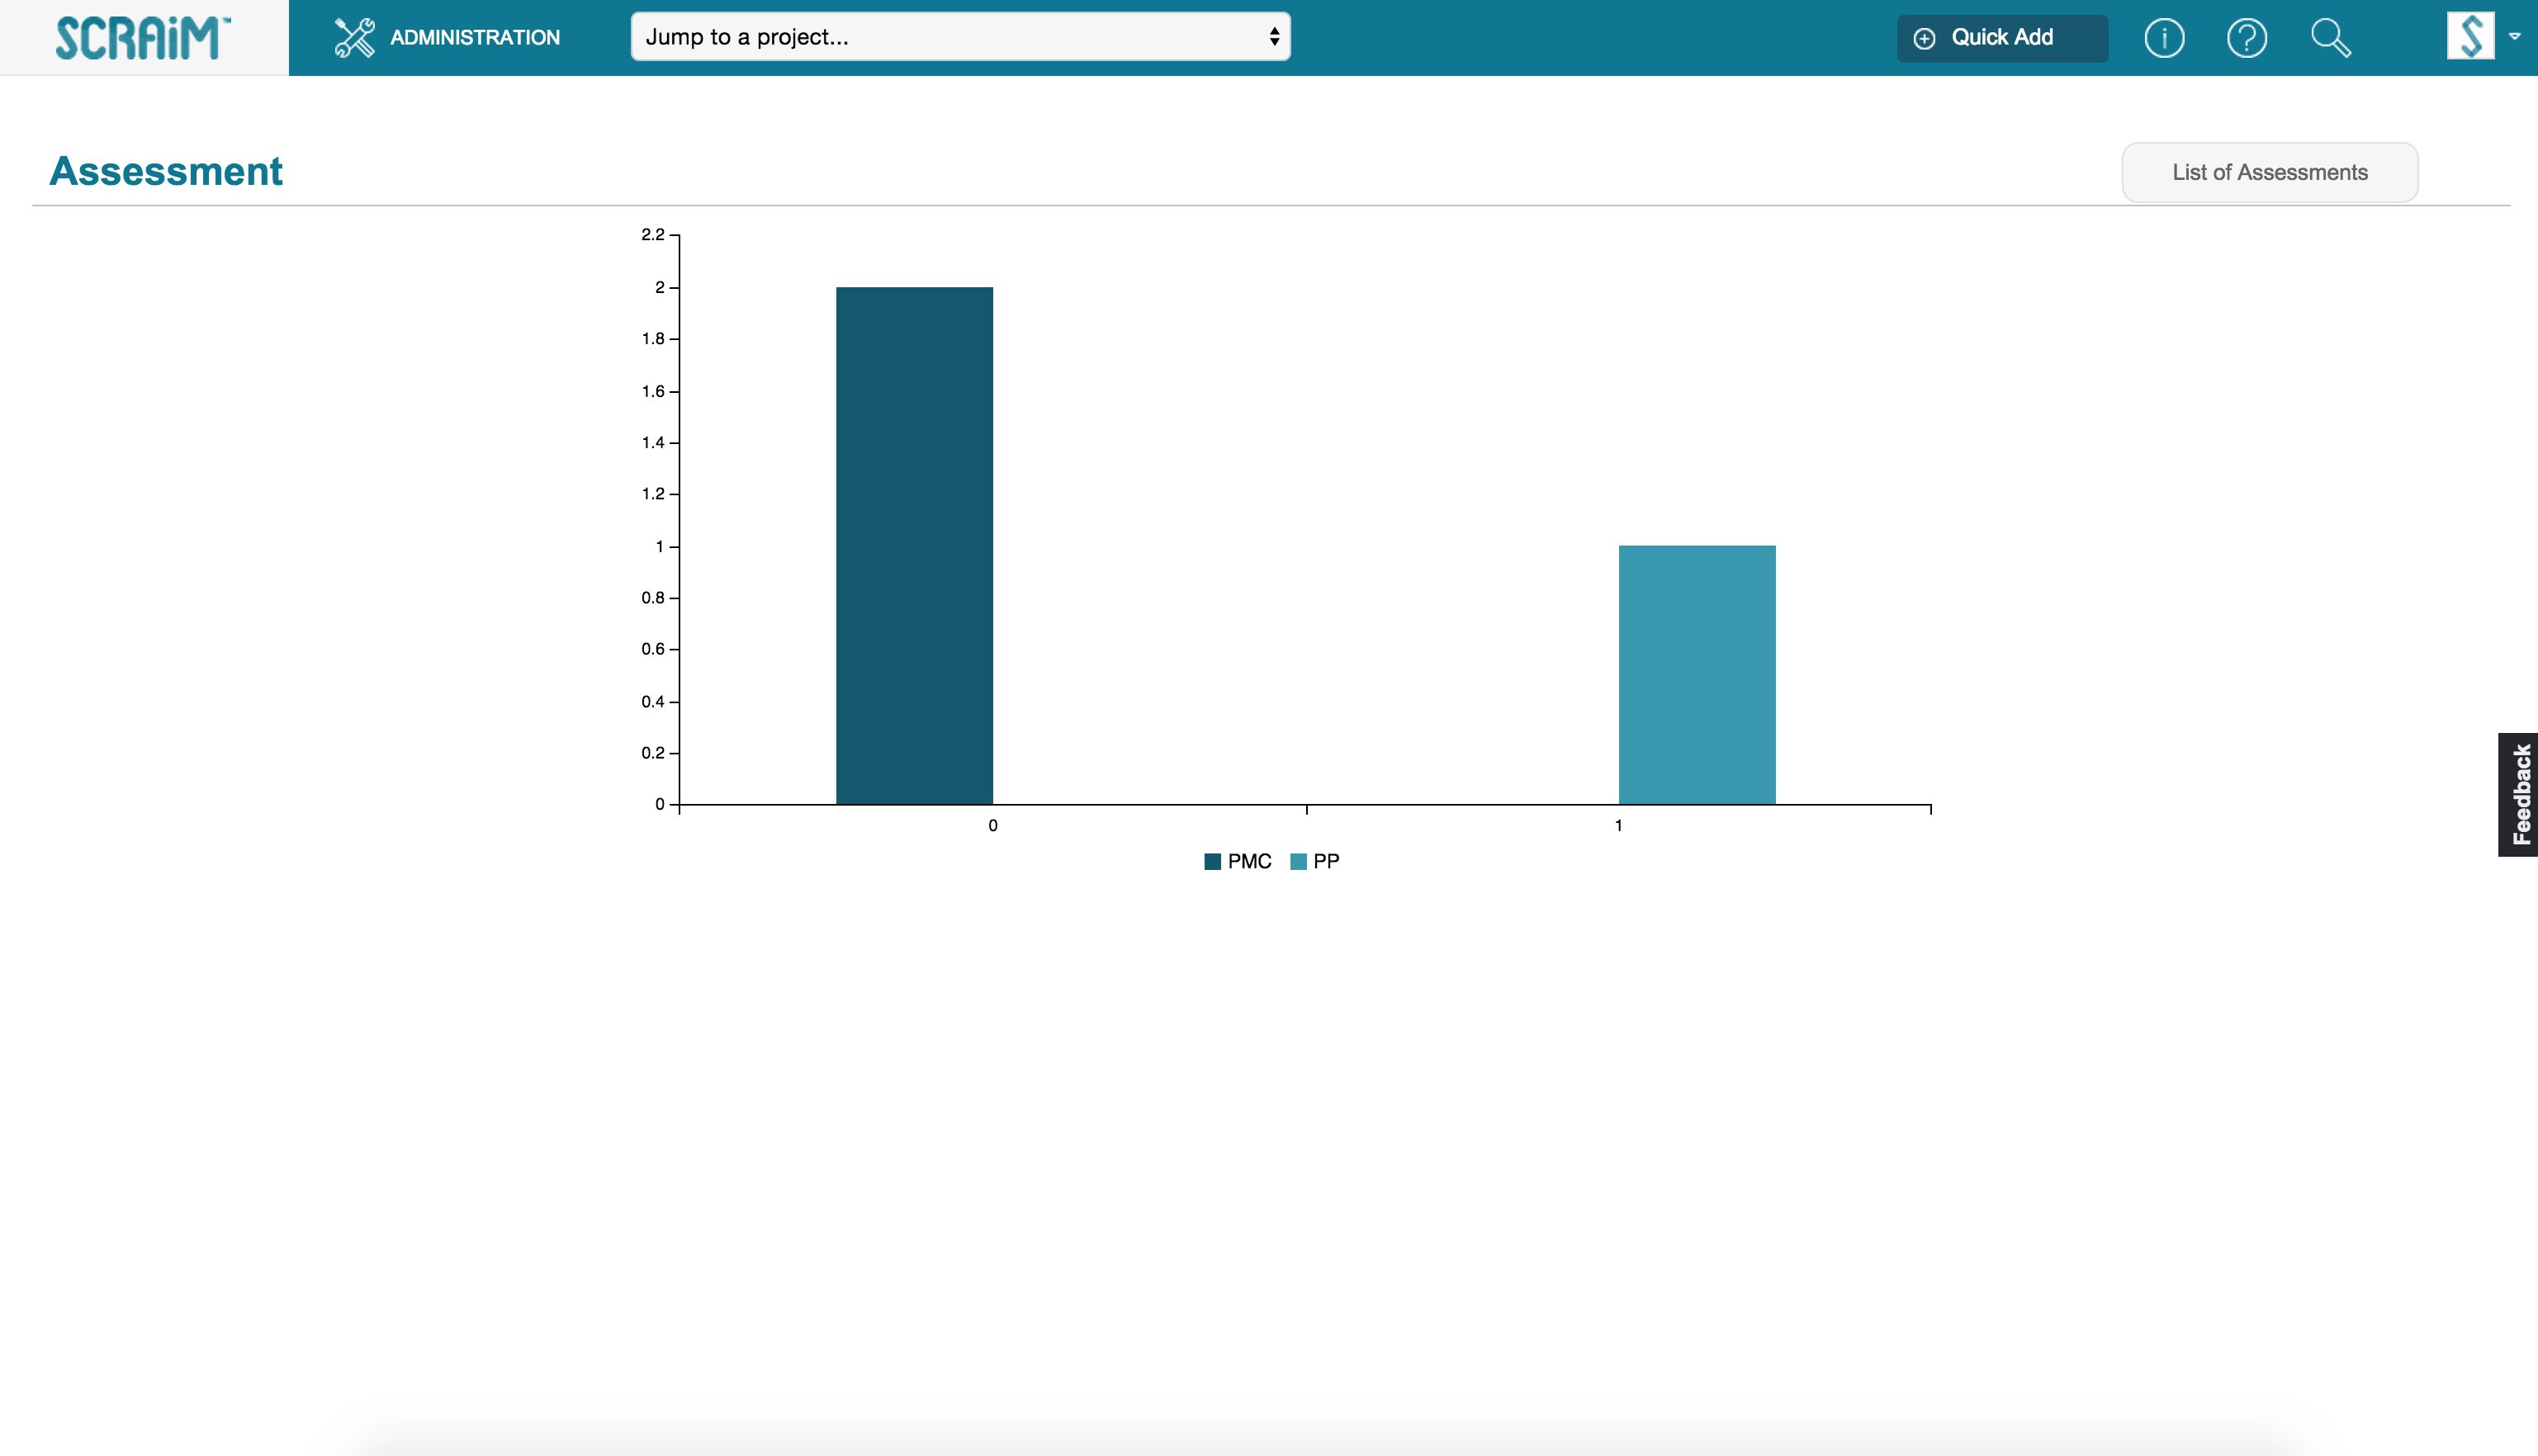
\includegraphics[width=0.9\textwidth]{area_view}
		\caption{Result of assessment, area view}
		\label{fig:area_view}
	\end{center}
\end{figure}

When inside the graph a certain process area is clicked, like for example PP which stands for Project Planning, the content of the graph changes to the practices results, as illustrated in \ref{fig:practices_view}.


\begin{figure}[!htb]
	\begin{center}
		\leavevmode
		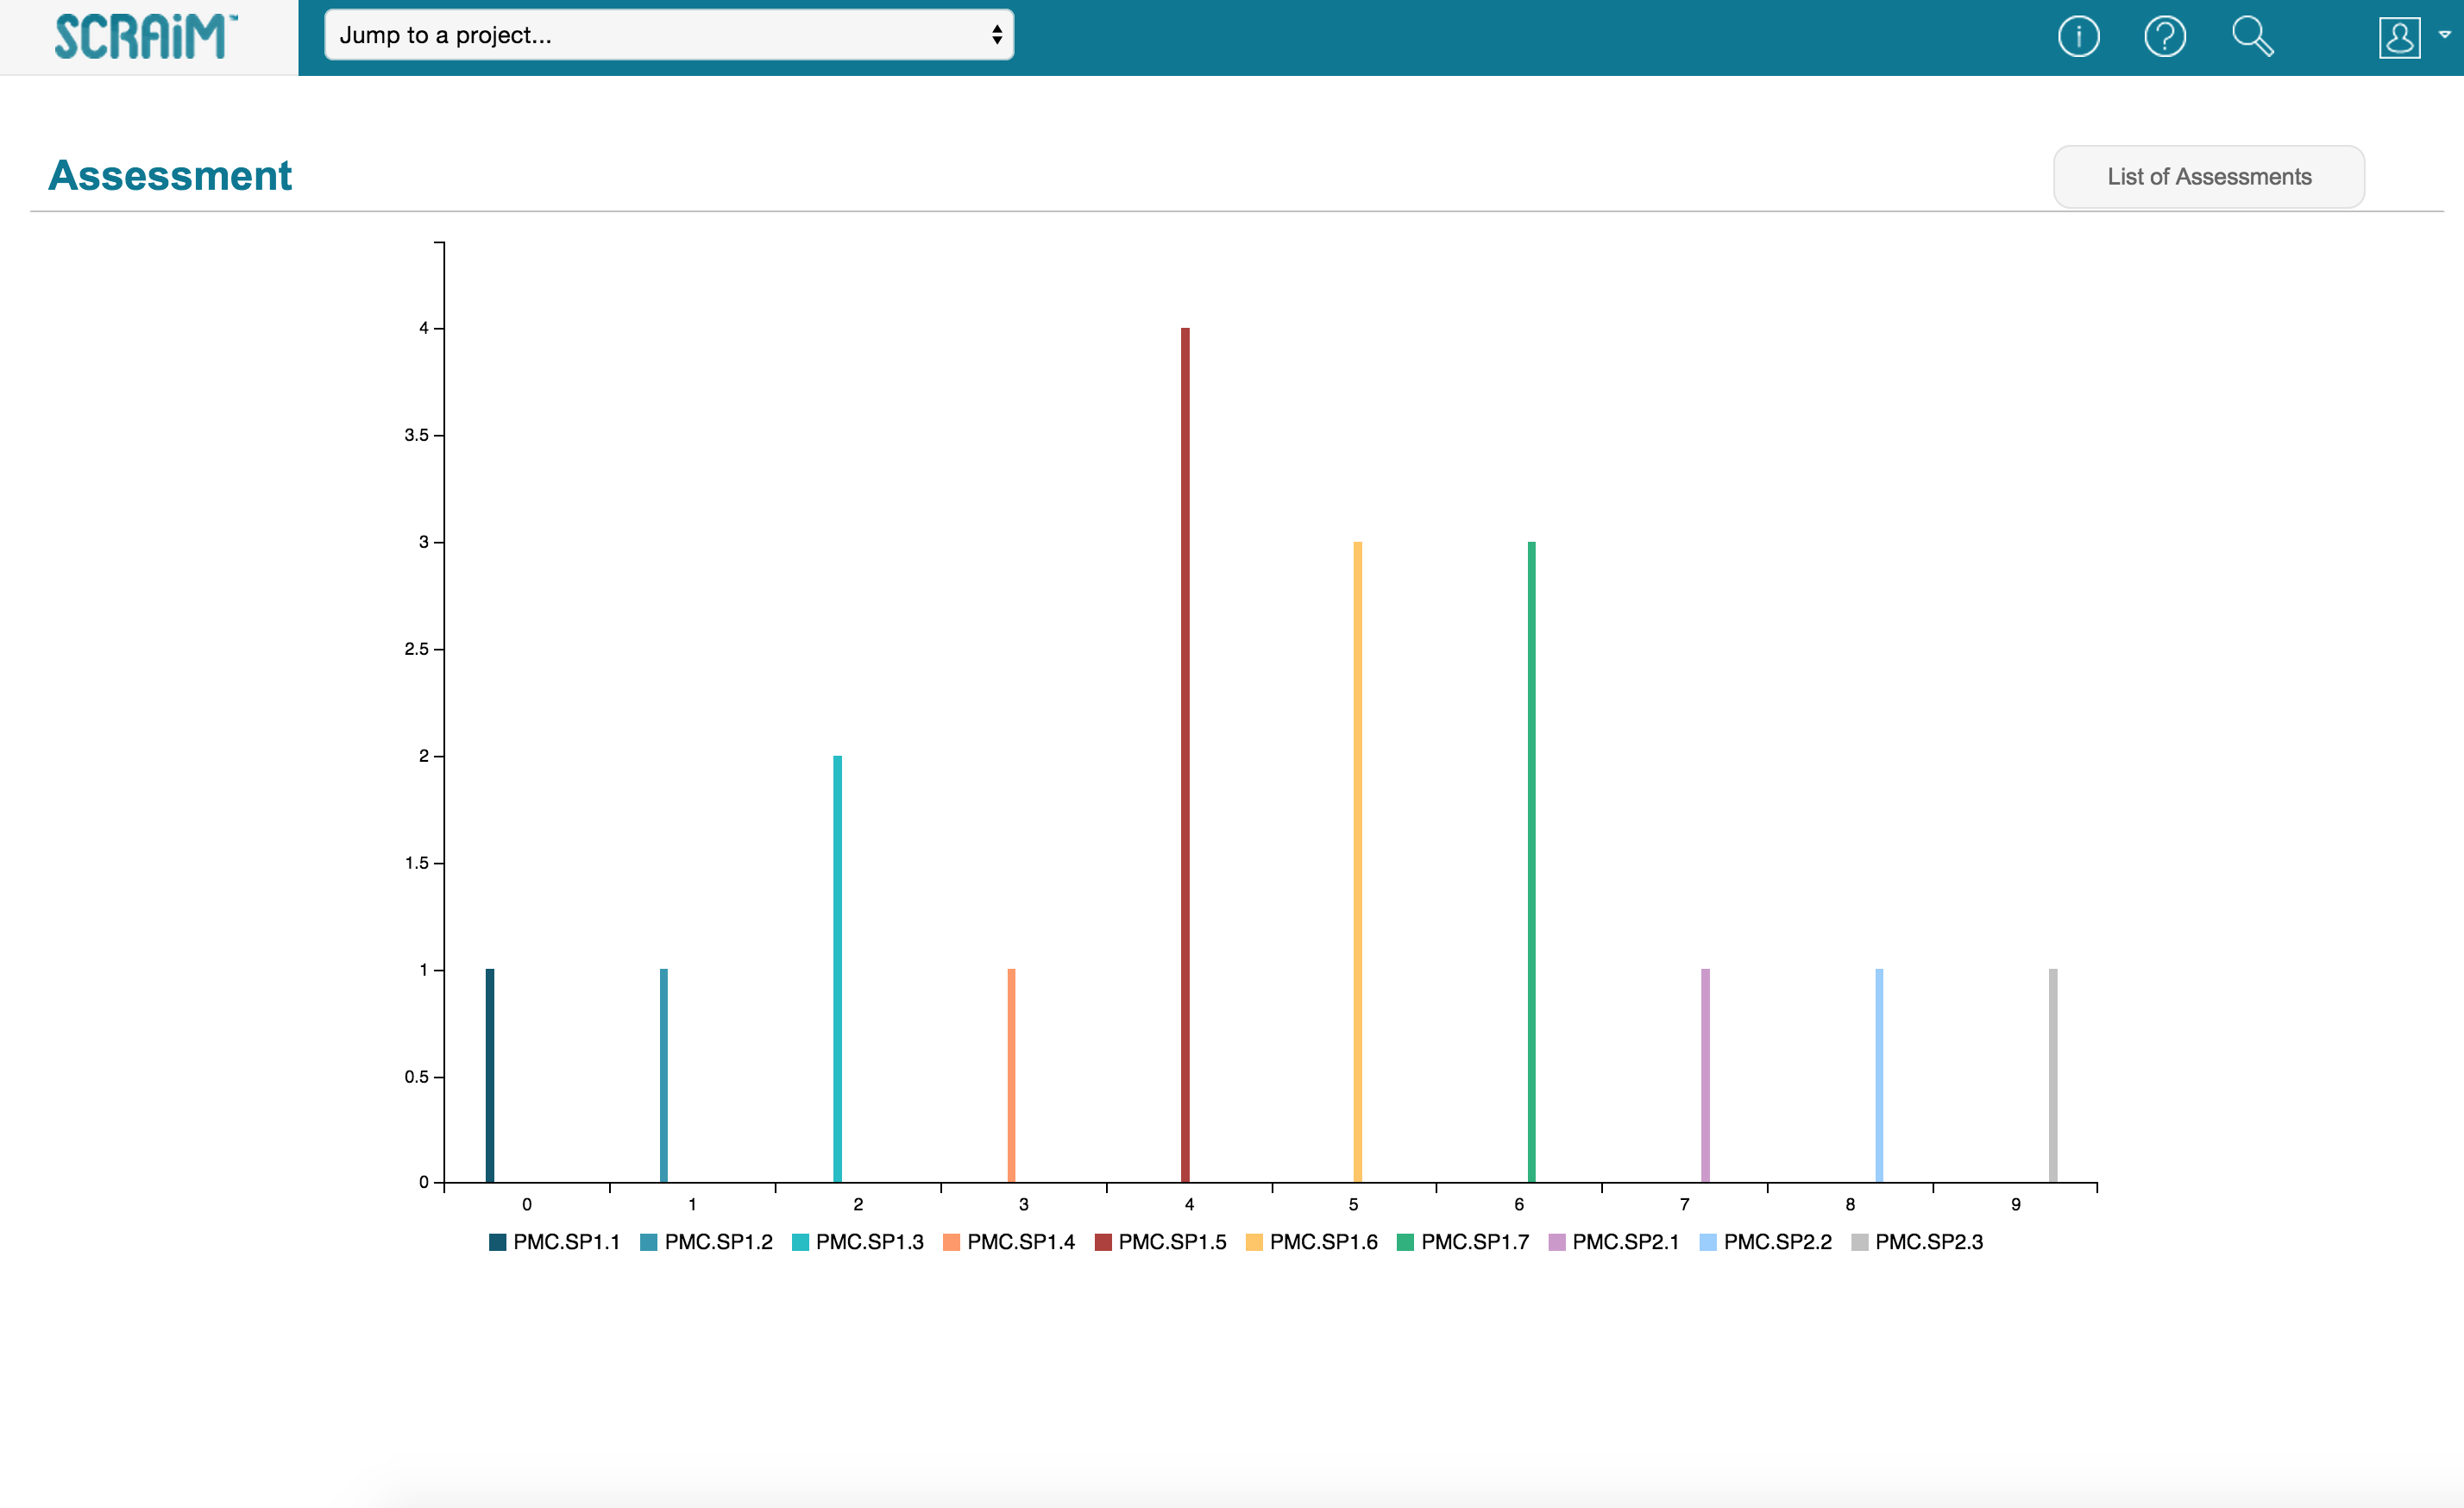
\includegraphics[width=0.9\textwidth]{practices_view}
		\caption{Result of assessment, practices view}
		\label{fig:practices_view}
	\end{center}
\end{figure}

It is possible to see more in detail the assessment result if the mouse cursor is over the bar that correspond to a practice. When that bar is clicked, it is shown in the page more information about that practice. Figure \ref{fig:practice_click}, shows us the information appended to the page when the Practice 1.1 of the first goal of Project Planning a	rea is clicked.

\begin{figure}[!htb]
	\begin{center}
		\leavevmode
		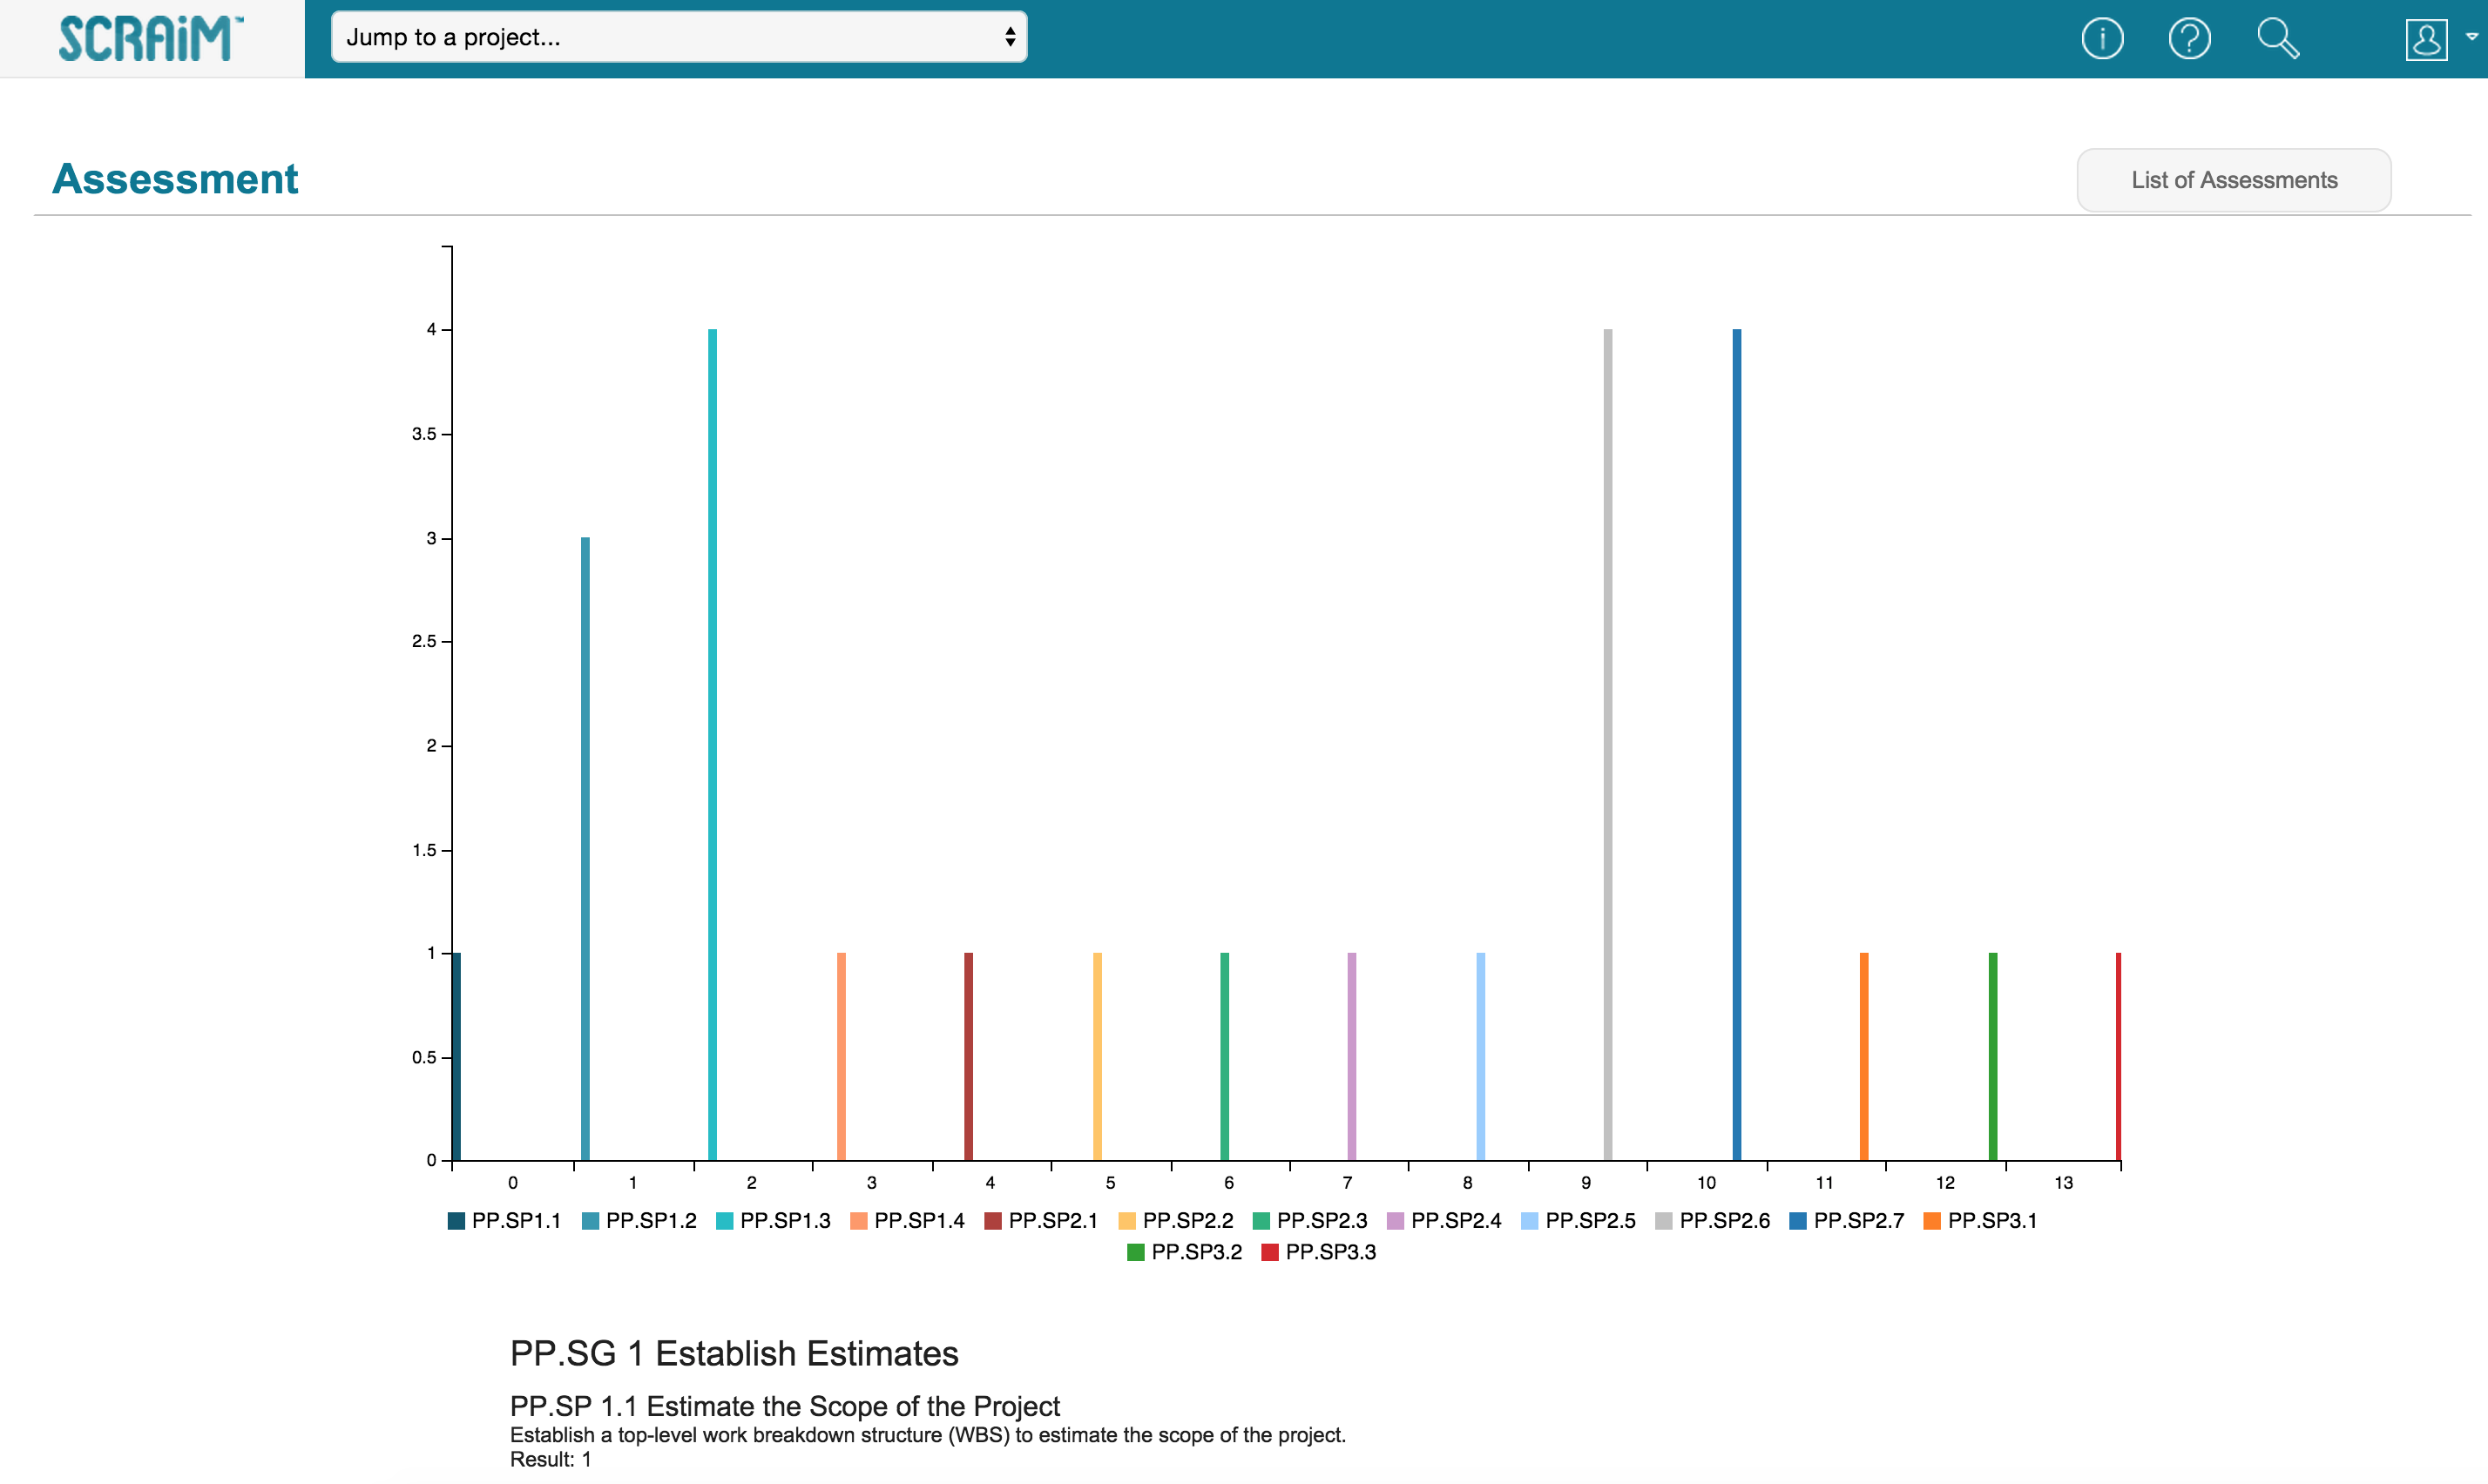
\includegraphics[width=0.9\textwidth]{practice_click}
		\caption{Result of assessment, practice view details}
		\label{fig:practice_click}
	\end{center}
\end{figure}

After all this process, all views allow the user to return to the Home screen, that contains the list of the assessments done. The assessment that we have done and we are seeing is already present on the list of assessments.
 
\section{Comparison between Automatic and Manual assessment} \label{sec:automatic}
%	Avaliação manual vs automatica trocar titulo

To determine if the implemented module is close to a real assessment is necessary to compare an automatic assessment (tool) to a manual assessment (human).

For that purpose is chosen a project that is already finished and instantiated in SCRAIM.
In both assessments that only the two areas featured in the implementation of this module are considered for this comparison.

\begin{figure}[!htb]
	\begin{center}
		\leavevmode
		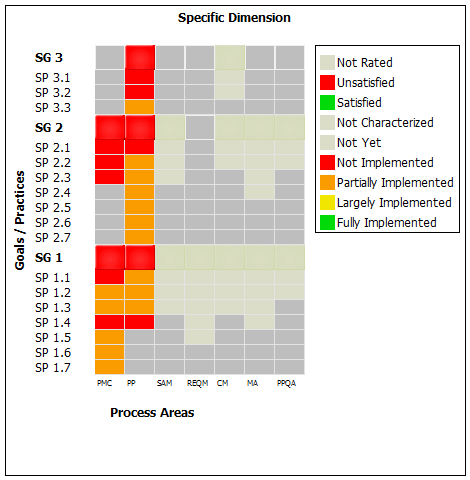
\includegraphics[width=0.9\textwidth]{manual_assessment}
		\caption{Manual assessment, done for one appraisal}
		\label{fig:manual_assessment}
	\end{center}
\end{figure}

\textbf{Manual Assessment}

The Manual assessment that is shown in Figure \ref{fig:manual_assessment} was performed by a Consultant from Strongstep.

In the manual assessment we can see that in Project Planing for the first goal only the last practice is not implemented and the others practices are Partially implemented. For the second goal all practices are partially implemented except the first one.
In the third goal only the last practice is partially implemented the others are not implemented.

For the area Project Monitoring and Control in the first goal the first and forth practices are classified as not implemented and the others as partially implemented. In the second goal all practices are not implemented.

\textbf{Automatic Assessment}

The Automatic assessment performed by the developed module can be seen in Figure \ref{fig:automatic_assessment}.

\begin{figure}[!htb]
	\begin{center}
		\leavevmode
		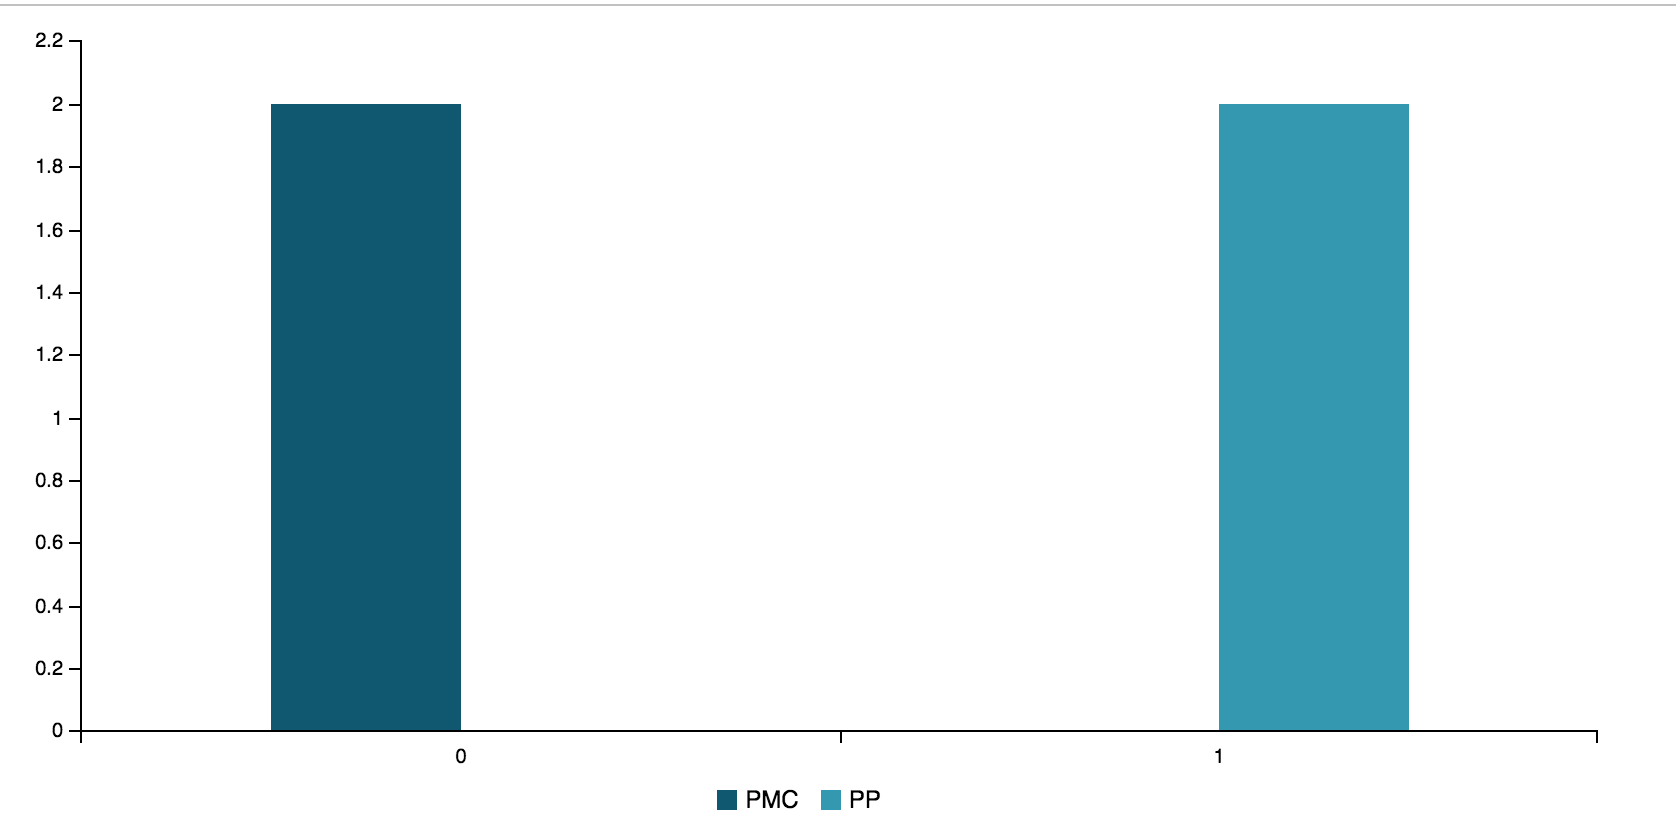
\includegraphics[width=0.9\textwidth]{automatic_assessment}
		\caption{Scraim Automatic Assessment}
		\label{fig:automatic_assessment}
	\end{center}
\end{figure}

In Figure \ref{fig:automatic_assessment} is presented the assessment of the two areas. In this case the assessment result for the areas of PP and PMC are 2 and 2 in the SCRAIM scale. That represent that is partially implemented.

For the PP area, the practices results are shown in Figure \ref{fig:results_pp}.

Using for method of approximation the scale presented in Section \ref{sec:mapping} and comparing the automatic results with the Manual assessment shown before one can conclude that in the most cases the mapping of the tool matched the manual assessment. In some cases like  the SP.2.2 the risks of the project weren't recorded on SCRAIM but in a document attached to the project.


Results for the PMC area are represented in Figure \ref{fig:results_pmc}. Using the same method that used before and comparing the two results, none practice stands out from the results, so the results are close to a real assessment.


\begin{figure}[!htb]
	\begin{center}
		\leavevmode
		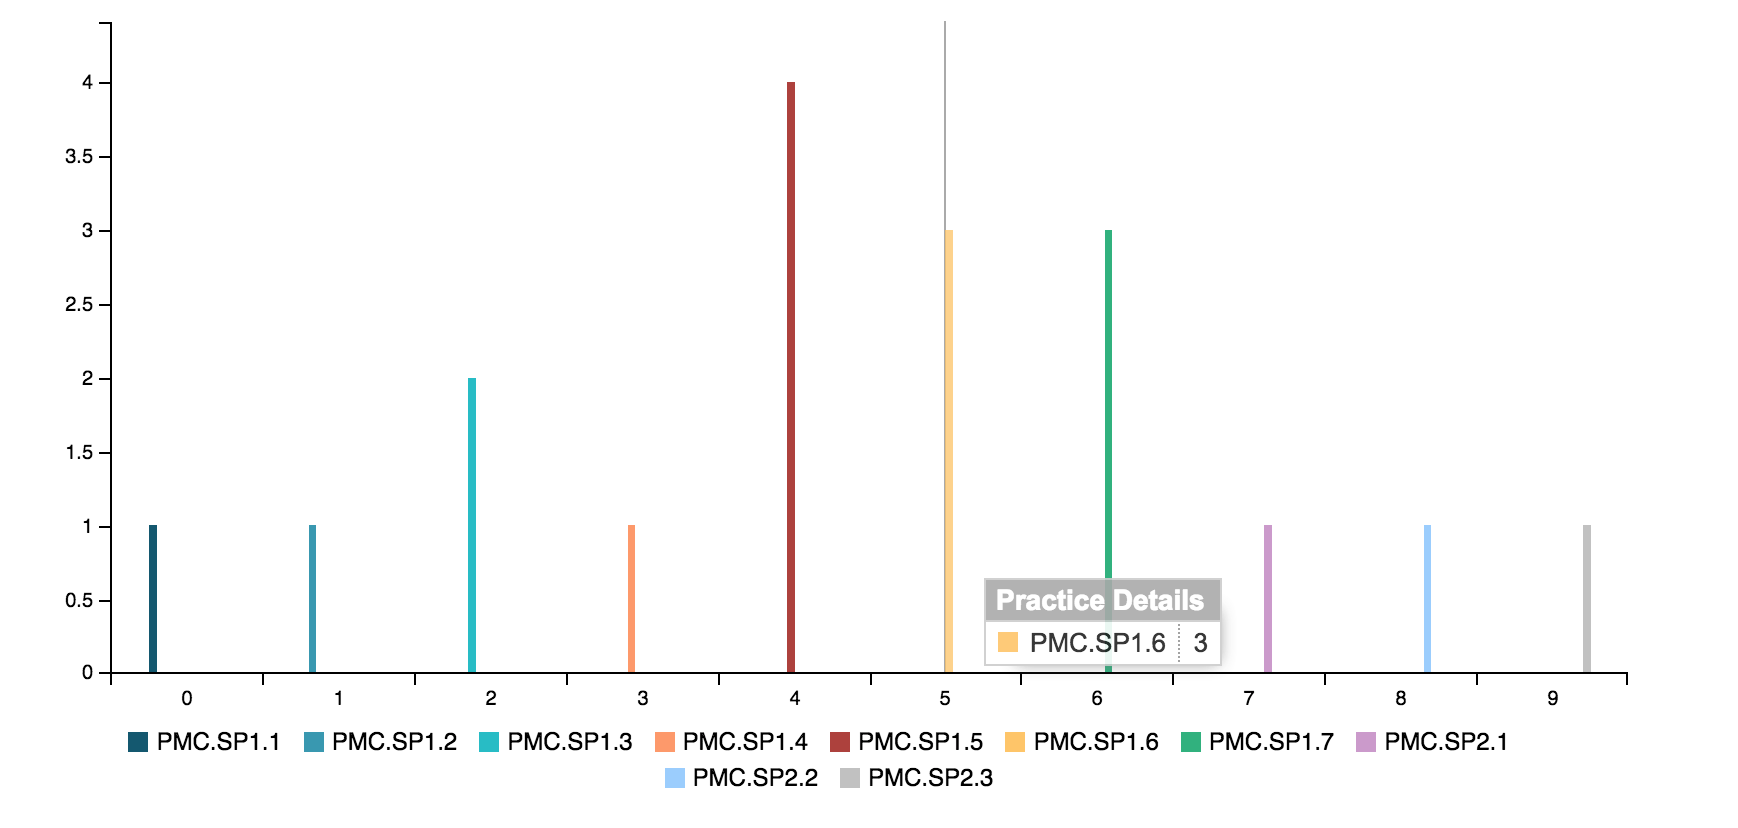
\includegraphics[width=0.9\textwidth]{results_pmc}
		\caption{Project Monitoring and Control Results}
		\label{fig:results_pp}
	\end{center}
\end{figure}

\begin{figure}[!htb]
	\begin{center}
		\leavevmode
		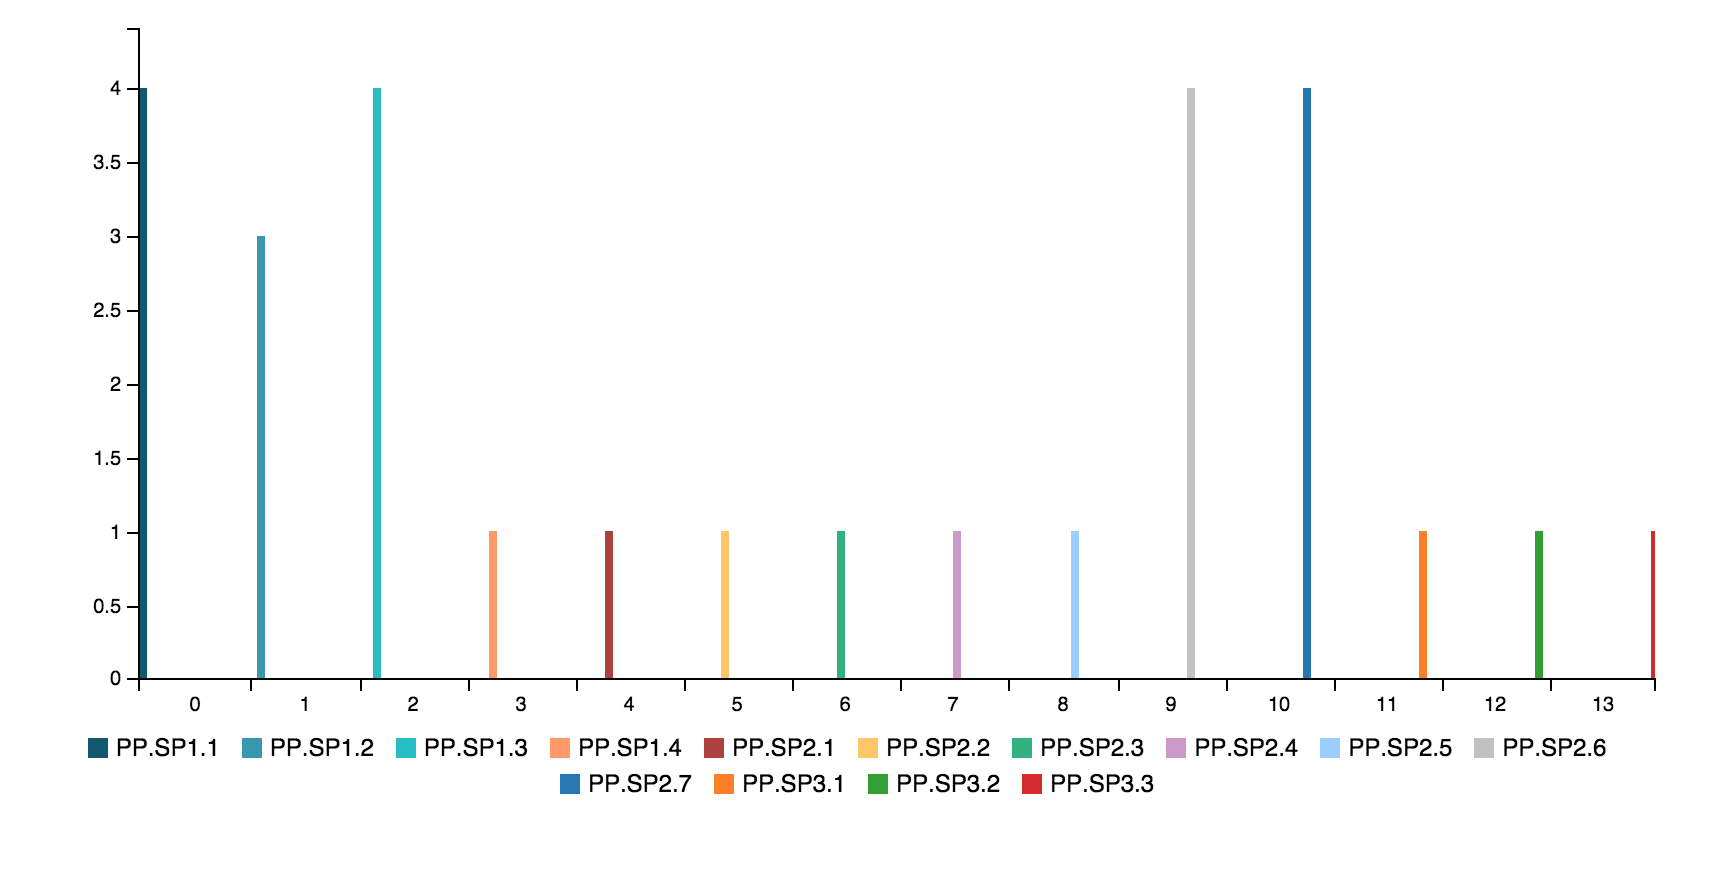
\includegraphics[width=0.9\textwidth]{results_pp}
		\caption{Project Planning Results}
		\label{fig:results_pmc}
	\end{center}
\end{figure}

In Table \ref{tab:automaticmanual} is presented side by side the results obtained. It must be used the scale map in Section \ref{sec:mapping}.

\begin{table}[h]
	\centering
	\caption{Automatic and Manual assessments}
	\begin{tabular}{|p{2cm}|p{3cm}|p{4cm}|}
		\hline
		Practice  & Automatic & Manual                \\
		\hline
		PP.SP 1.1 & 4         & Partially Implemented \\
		PP.SP 1.2 & 3         & Partially Implemented \\
		PP.SP 1.3 & 4         & Partially Implemented \\
		PP.SP 1.4 & 1         & Not Implemented       \\
		PP.SP 2.1 & 1         & Not Implemented       \\
		PP.SP 2.2 & 1         & Partially Implemented \\
		PP.SP 2.3 & 1         & Partially Implemented \\
		PP.SP 2.4 & 1         & Partially Implemented \\
		PP.SP 2.5 & 1         & Partially Implemented \\
		PP.SP 2.6 & 4         & Partially Implemented \\
		PP.SP 2.7 & 4         & Partially Implemented \\
		PP.SP 3.1 & 1         & Not Implemented       \\
		PP.SP 3.2 & 1         & Not Implemented       \\
		PP.SP 3.3 & 1         & Partially Implemented\\
		PMC.SP 1.1 & 1 & Not Implemented       \\
		PMC.SP 1.2 & 1 & Partially Implemented \\
		PMC.SP 1.3 & 2 & Partially Implemented \\
		PMC.SP 1.4 & 1 & Not Implementd        \\
		PMC.SP 1.5 & 4 & Partially Implemented \\
		PMC.SP 1.6 & 3 & Partially Implemented \\
		PMC.SP 1.7 & 3 & Partially Implemented \\
		PMC.SP 2.1 & 1 & Not Implementd        \\
		PMC.SP 2.2 & 1 & Not Implementd        \\
		PMC.SP 2.3 & 1 & Not Implementd        \\
		\hline
	\end{tabular}
	\label{tab:automaticmanual}
\end{table}